\documentclass[13pt,a4paper]{article}
\usepackage{a4wide,amssymb,epsfig,latexsym,multicol,array,hhline,fancyhdr}
\usepackage{amsmath}
\usepackage{lastpage}
\usepackage[lined,boxed,commentsnumbered]{algorithm2e}
\usepackage{enumerate}
\usepackage{color}
\usepackage{graphicx}							% Standard graphics package
\usepackage{array}
\usepackage{tabularx, caption}
\usepackage{multirow}
\usepackage{multicol}
\usepackage{rotating}
\usepackage{graphics}
\usepackage{geometry}
\usepackage{setspace}
\usepackage{epsfig}
\usepackage{tikz}
\usetikzlibrary{arrows,snakes,backgrounds}
\usepackage{hyperref}
\hypersetup{urlcolor=blue,linkcolor=black,citecolor=black,colorlinks=true} 
%\usepackage{pstcol} 								% PSTricks with the standard color package

\newtheorem{theorem}{{\bf Theorem}}
\newtheorem{property}{{\bf Property}}
\newtheorem{proposition}{{\bf Proposition}}
\newtheorem{corollary}[proposition]{{\bf Corollary}}
\newtheorem{lemma}[proposition]{{\bf Lemma}}

\AtBeginDocument{\renewcommand*\contentsname{Contents}}
\AtBeginDocument{\renewcommand*\refname{References}}
%\usepackage{fancyhdr}
\setlength{\headheight}{40pt}
\pagestyle{fancy}
\fancyhead{} % clear all header fields
\fancyhead[L]{
	\begin{tabular}{rl}
		\begin{picture}(25,15)(0,0)
			\put(0,-8){
\includegraphics[width=8mm, height=8mm]{hcmut.png}}
			%\put(0,-8){\epsfig{width=10mm,figure=hcmut.eps}}
		\end{picture}&
		%
\includegraphics[width=8mm, height=8mm]{hcmut.png} & %
		\begin{tabular}{l}
			\textbf{\bf \ttfamily University of Technology, Ho Chi Minh City}\\
			\textbf{\bf \ttfamily Faculty of Computer Science and Engineering}
		\end{tabular} 	
	\end{tabular}
}
\fancyhead[R]{
	\begin{tabular}{l}
		\tiny \bf \\
		\tiny \bf 
\end{tabular}  }
\fancyfoot{} % clear all footer fields
\fancyfoot[L]{\scriptsize \ttfamily Homework for Embedded System Processing year 2020 - 2021}
\fancyfoot[R]{\scriptsize \ttfamily Page {\thepage}/\pageref{LastPage}}
\renewcommand{\headrulewidth}{0.3pt}
\renewcommand{\footrulewidth}{0.3pt}


%%%
\setcounter{secnumdepth}{4}
\setcounter{tocdepth}{3}
\makeatletter
\newcounter {subsubsubsection}[subsubsection]
\renewcommand\thesubsubsubsection{\thesubsubsection .\@alph\c@subsubsubsection}
\newcommand\subsubsubsection{\@startsection{subsubsubsection}{4}{\z@}%
	{-3.25ex\@plus -1ex \@minus -.2ex}%
	{1.5ex \@plus .2ex}%
	{\normalfont\normalsize\bfseries}}
\newcommand*\l@subsubsubsection{\@dottedtocline{3}{10.0em}{4.1em}}
\newcommand*{\subsubsubsectionmark}[1]{}
\makeatother

\begin{document}
	
	\begin{titlepage}
		\begin{center}
			VIETNAM NATIONAL UNIVERSITY, HO CHI MINH CITY \\
			UNIVERSITY OF TECHNOLOGY \\
			FACULTY OF COMPUTER SCIENCE AND ENGINEERING
		\end{center}
		
		\vspace{1cm}
		
		\begin{figure}[h!]
			\begin{center}
				
\includegraphics[width=3cm]{hcmut.png}
			\end{center}
		\end{figure}
		
		\vspace{1cm}
		
		\begin{center}
			\color{blue}
			\begin{tabular}{c}
				\multicolumn{1}{l}{\textbf{\centerline{{\Huge EMBEDDED SYSTEMS}}}}\\
				~~\\
				\hline
				\\
				\multicolumn{1}{l}{\textbf{\centerline{{\LARGE Homework Result}}}}\\
				\\
				\textbf{{\huge State Machine Model for Washing Machine}}\\
				\\
				\hline
			\end{tabular}
			\color{blue}
		\end{center}
		\vspace{1cm}
		
		\begin{table}[h]
			\color{blue}
			\begin{tabular}{rrl}
				\hspace{5 cm} & Advisor: & Pham Hoang Anh\\
				& Students: & Tran Long Vi - 1814804 \\
			\end{tabular}
			\color{blue}
		\end{table}
		
		\vspace{4 cm}
		\begin{center}
			{\footnotesize\large HO CHI MINH CITY, APRIL 2021}
		\end{center}
	\end{titlepage}
	
	
	%\thispagestyle{empty}
	\newpage
	
	
	%%%%%%%%%%%%%%%%%%%%%%%%%%%%%%%%%
	\section{STATE-MACHINE DIAGRAM}
	\begin{figure}[h!]
		\begin{center}
			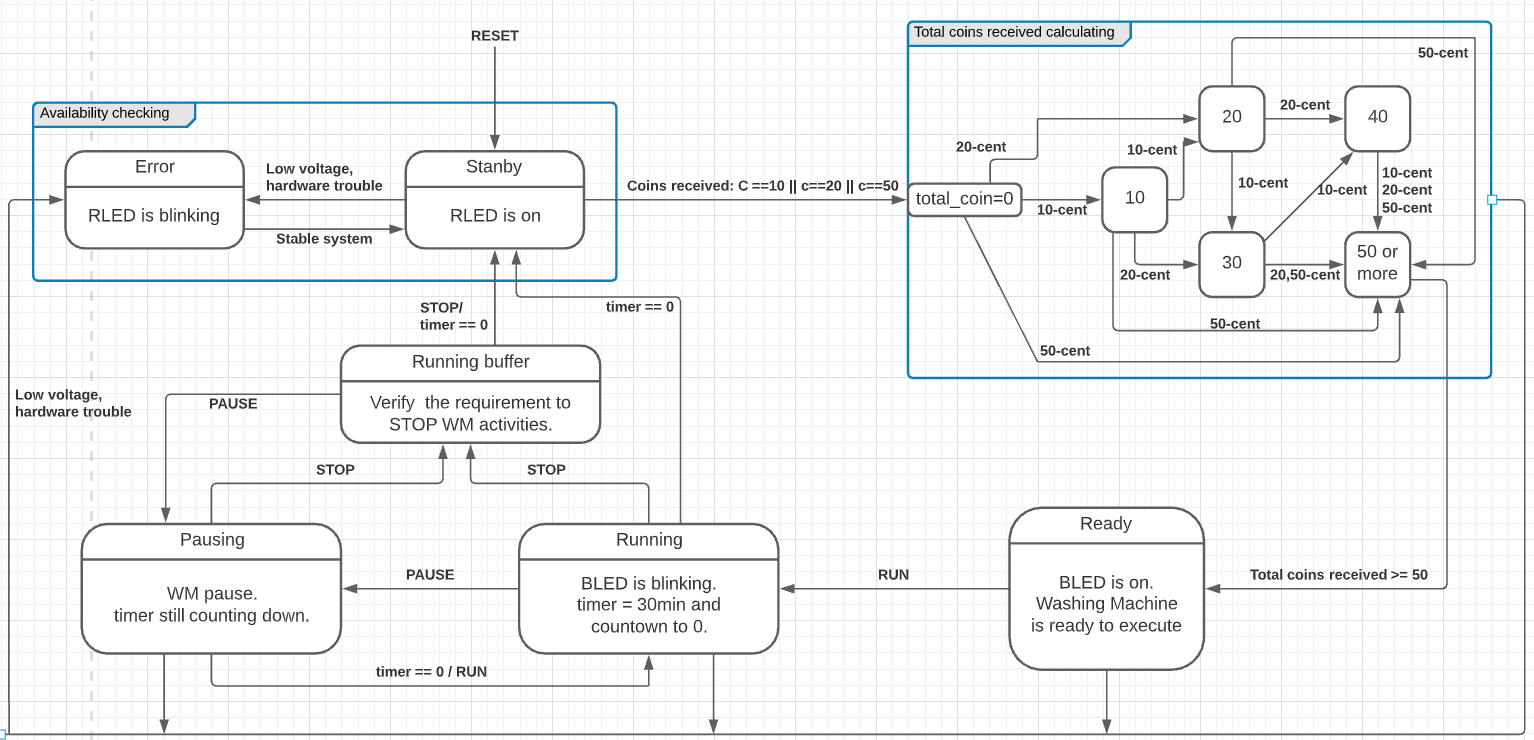
\includegraphics[width=17cm]{diagram.png}
			\caption{\textit{State-Machine Diagram for Washing Machine}}
		\end{center}
	\end{figure} 
	\section{DETAILED ANALYSIS OF THIS SYSTEM}
	\begin{enumerate}
		\item[$\bullet$] Availability checking block: this block is used to check the availability of the Washing Machine, by: 
			\begin{enumerate}
				\item[$\circ$] If this system is available to serve, the current statement is \textit{Stanby}. System can't execute any processes (Except \textit{Error} state) if it never cross \textit{Stanby} state before.
				\item[$\circ$] If this system has problems that affects to activities of system (like low voltage,corrupted components,...), the current statement is \textit{Error}. By all other state, the state will change to \textit{Error} whenever the system is down or running incorrectly in comparison to the algorithm.
			\end{enumerate}
		\item[$\bullet$] Total coins received calculating block: This block is used to calculate and send feedback that system had received enough coin ($total\_coin \geq 50$).This block is created base on the rules:
			\begin{enumerate}
				\item[$\circ$] This block only accepts 10-cent, 20 cent and 50-cent coins.
				\item[$\circ$] If customer use other denominations, system will still receive coins but $total\_coin$ doesn't change.
				\item[$\circ$] System has no service provided to return excess cash if $total\_coin \geq 50$.
			\end{enumerate}
		\item[$\bullet$] \textit{Ready} state: this state is executed if and only if $total\_coin \geq 50$. In this state, system must wait for customer requirement by press \textit{RUN} button.
		\item[$\bullet$] \textit{Running} state: this state is activated when customer press button \textit{RUN} in \textit{Ready} state. 
			\begin{enumerate}
				\item[$\circ$] A value $timer$ is initiated to countdown from min 30 to 0, this is the maximum time the system processes a washing process required by customer.
				\item[$\circ$] If $timer = 0$, system will go to \textit{Stanby} state to wait next requirement.
				\item[$\circ$] if \textit{PAUSE} button is pressed, system will go to \textit{Pausing} state.
			\end{enumerate}	
		\item[$\bullet$] \textit{Pausing} state: this state is used to pause the system execution when \textit{PAUSE} button is pressed. \\
		In this state, $timer$ is still counting down. If $timer = 0$ or RUN button is pressed, system will go back to \textit{Running} state.
		\item[$\bullet$] If for some reason, customer wanna stop the system execution, he/she has just pressed \textit{STOP} button double time. 
			\begin{enumerate}
				\item[$\circ$] At the first press (System is in \textit{Running} state or \textit{Pausing} state), system will change to \textit{Running Buffer} state. 
				\item[$\circ$] \textit{Running Buffer} state is the same function as \textit{Running} state, but it provides the customer with the function of stopping the system from executing without waiting for $time = 0$.
			\end{enumerate}
	\end{enumerate}
\end{document}